% ===================== Extrapolations to the physical limit (thesis Ch. 7) =====================
\section{Extrapolations to the physical limit}

\begin{frame}{Extrapolations to the physical limit}
  \begin{columns}[c]
    \begin{column}{0.46\textwidth}\centering
      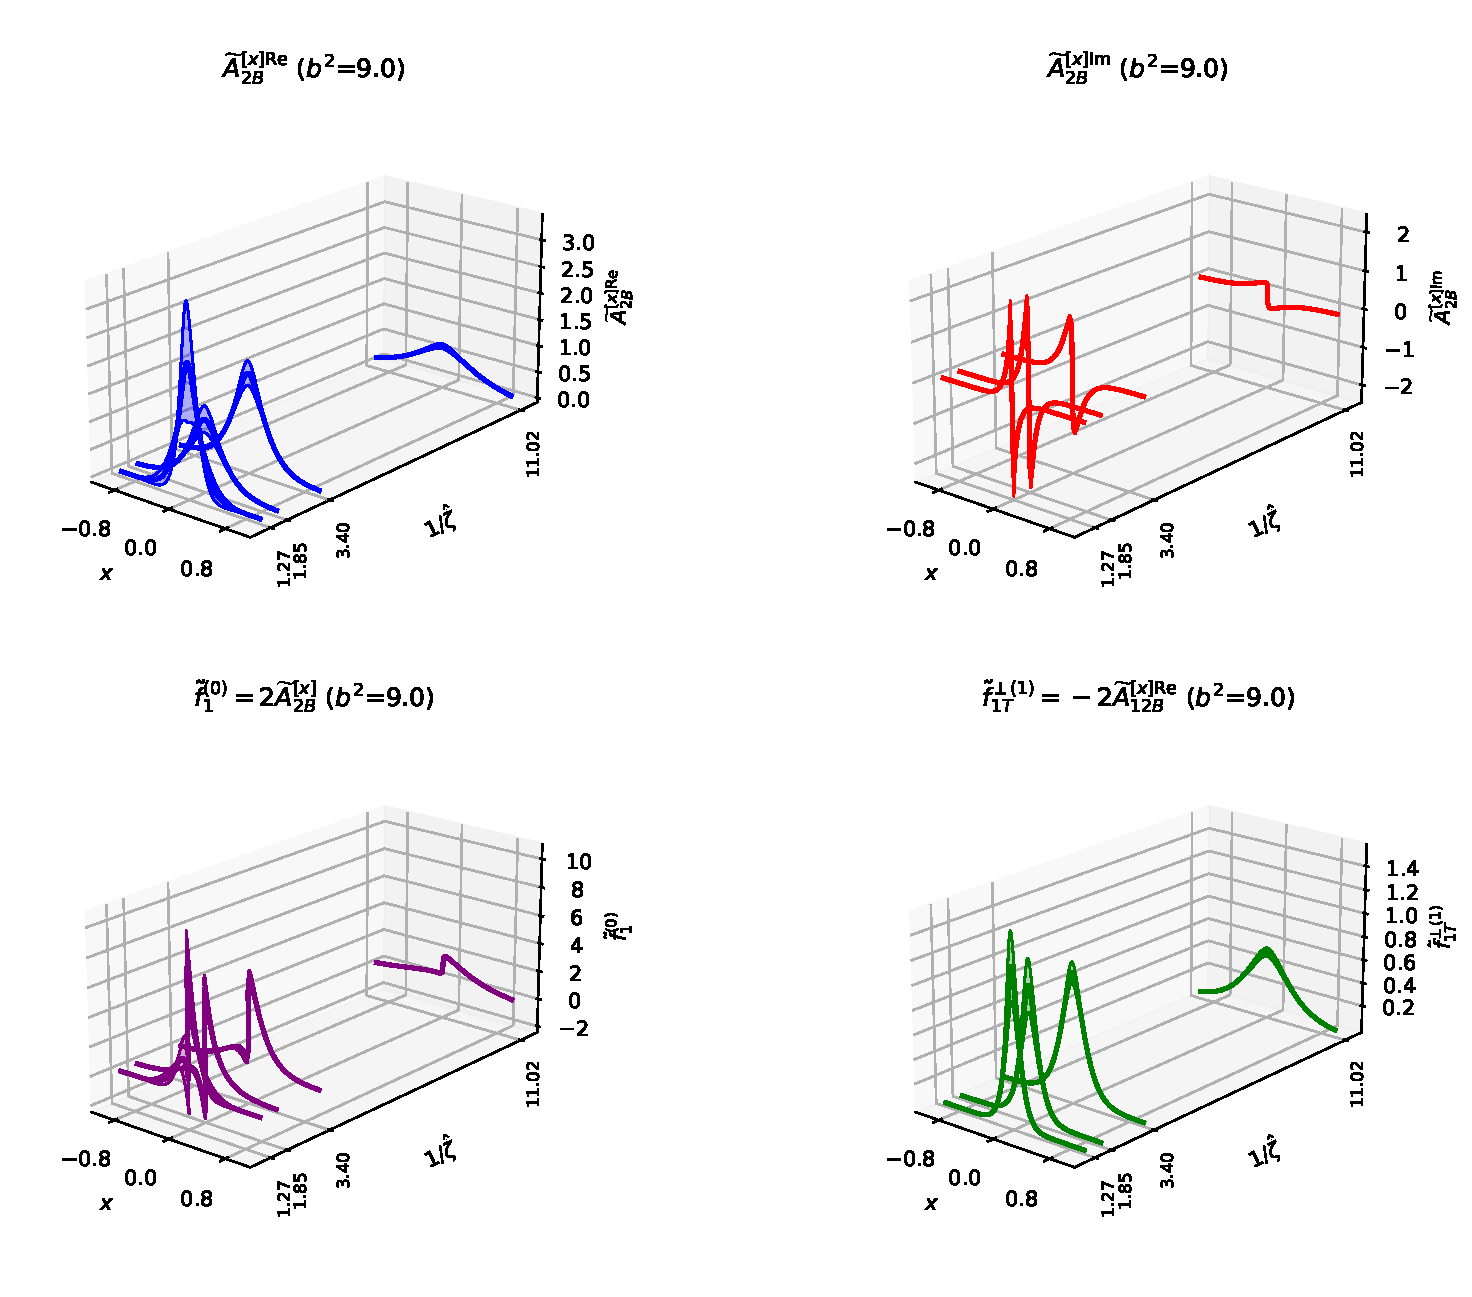
\includegraphics[width=\linewidth,height=0.6\textheight,keepaspectratio]{SimulFit_Distinct_1_over_PL_bmin3_eta610_b29.0_Amps.pdf}
    \end{column}
    \begin{column}{0.52\textwidth}\centering
      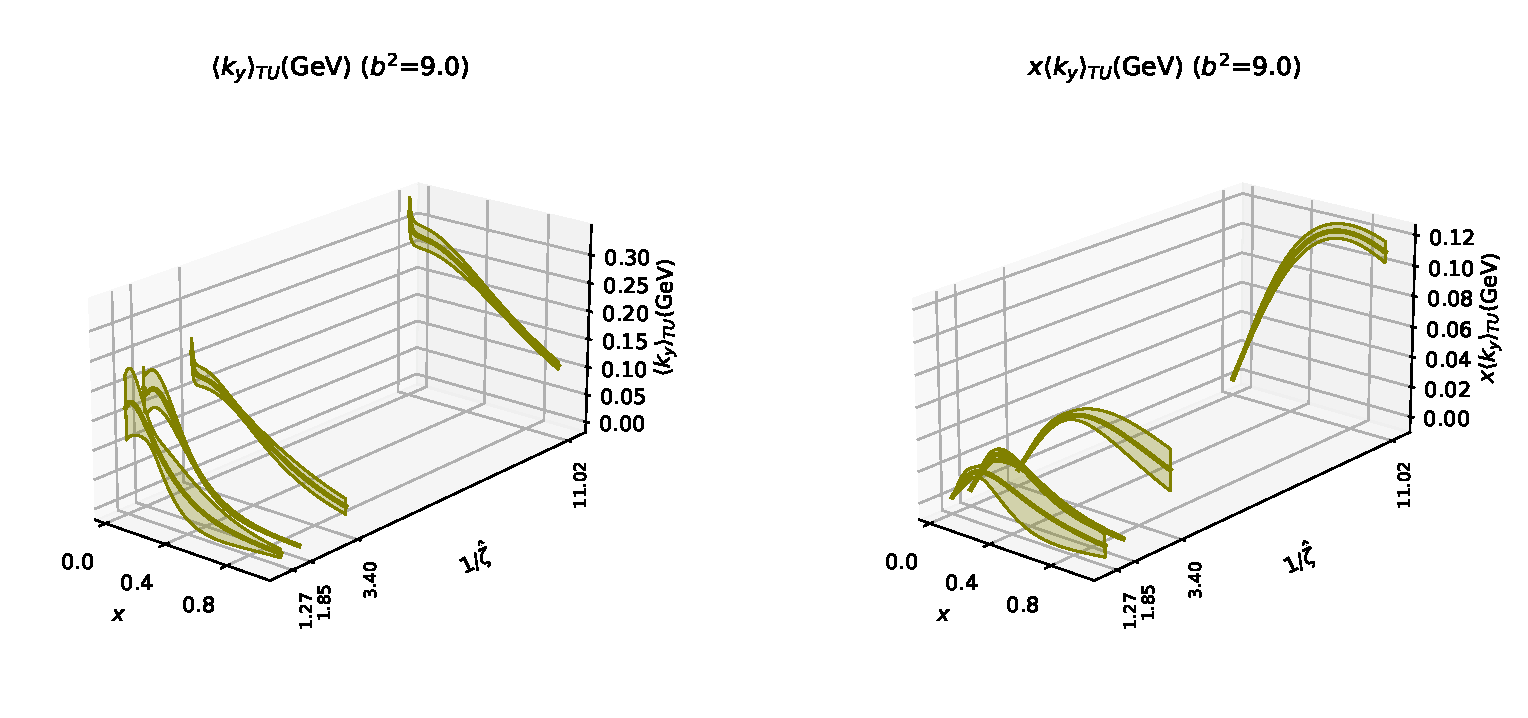
\includegraphics[width=\linewidth,height=0.6\textheight,keepaspectratio]{SimulFit_Distinct_1_over_PL_bmin3_eta610_b29.0_Sivers.pdf}
    \end{column}
  \end{columns}
  {\scriptsize Left: discrete $\hat\zeta$ slices of $\tAmp^{[x]\text{Re}}_{2B}$, $\tAmp^{[x]\text{Im}}_{2B}$, $\tilde f_1^{(0)}=2\tAmp^{[x]}_{2B}$ and $\tilde f_{1T}^{\perp(1)}=-2\tAmp^{[x]\text{Re}}_{12B}$ against $x$ and $1/\hat\zeta$ at $|b_T|=3a\approx0.34$ fm; one ribbon per momentum $P_L=-1,\dots,-4$ ($1/\hat\zeta=11.02,3.40,1.85,1.27$). The drift with $1/\hat\zeta$ motivates the extrapolation $\hat\zeta\to\infty$.
  Right: Sivers shift $\langle k_y\rangle_{TU}$ and $x\langle k_y\rangle_{TU}$ for the same momenta and $|b_T|$, restricted to $x\ge0$.}
\end{frame}

\begin{frame}{Extrapolation $\zetahat\to\infty$}
  \centering
  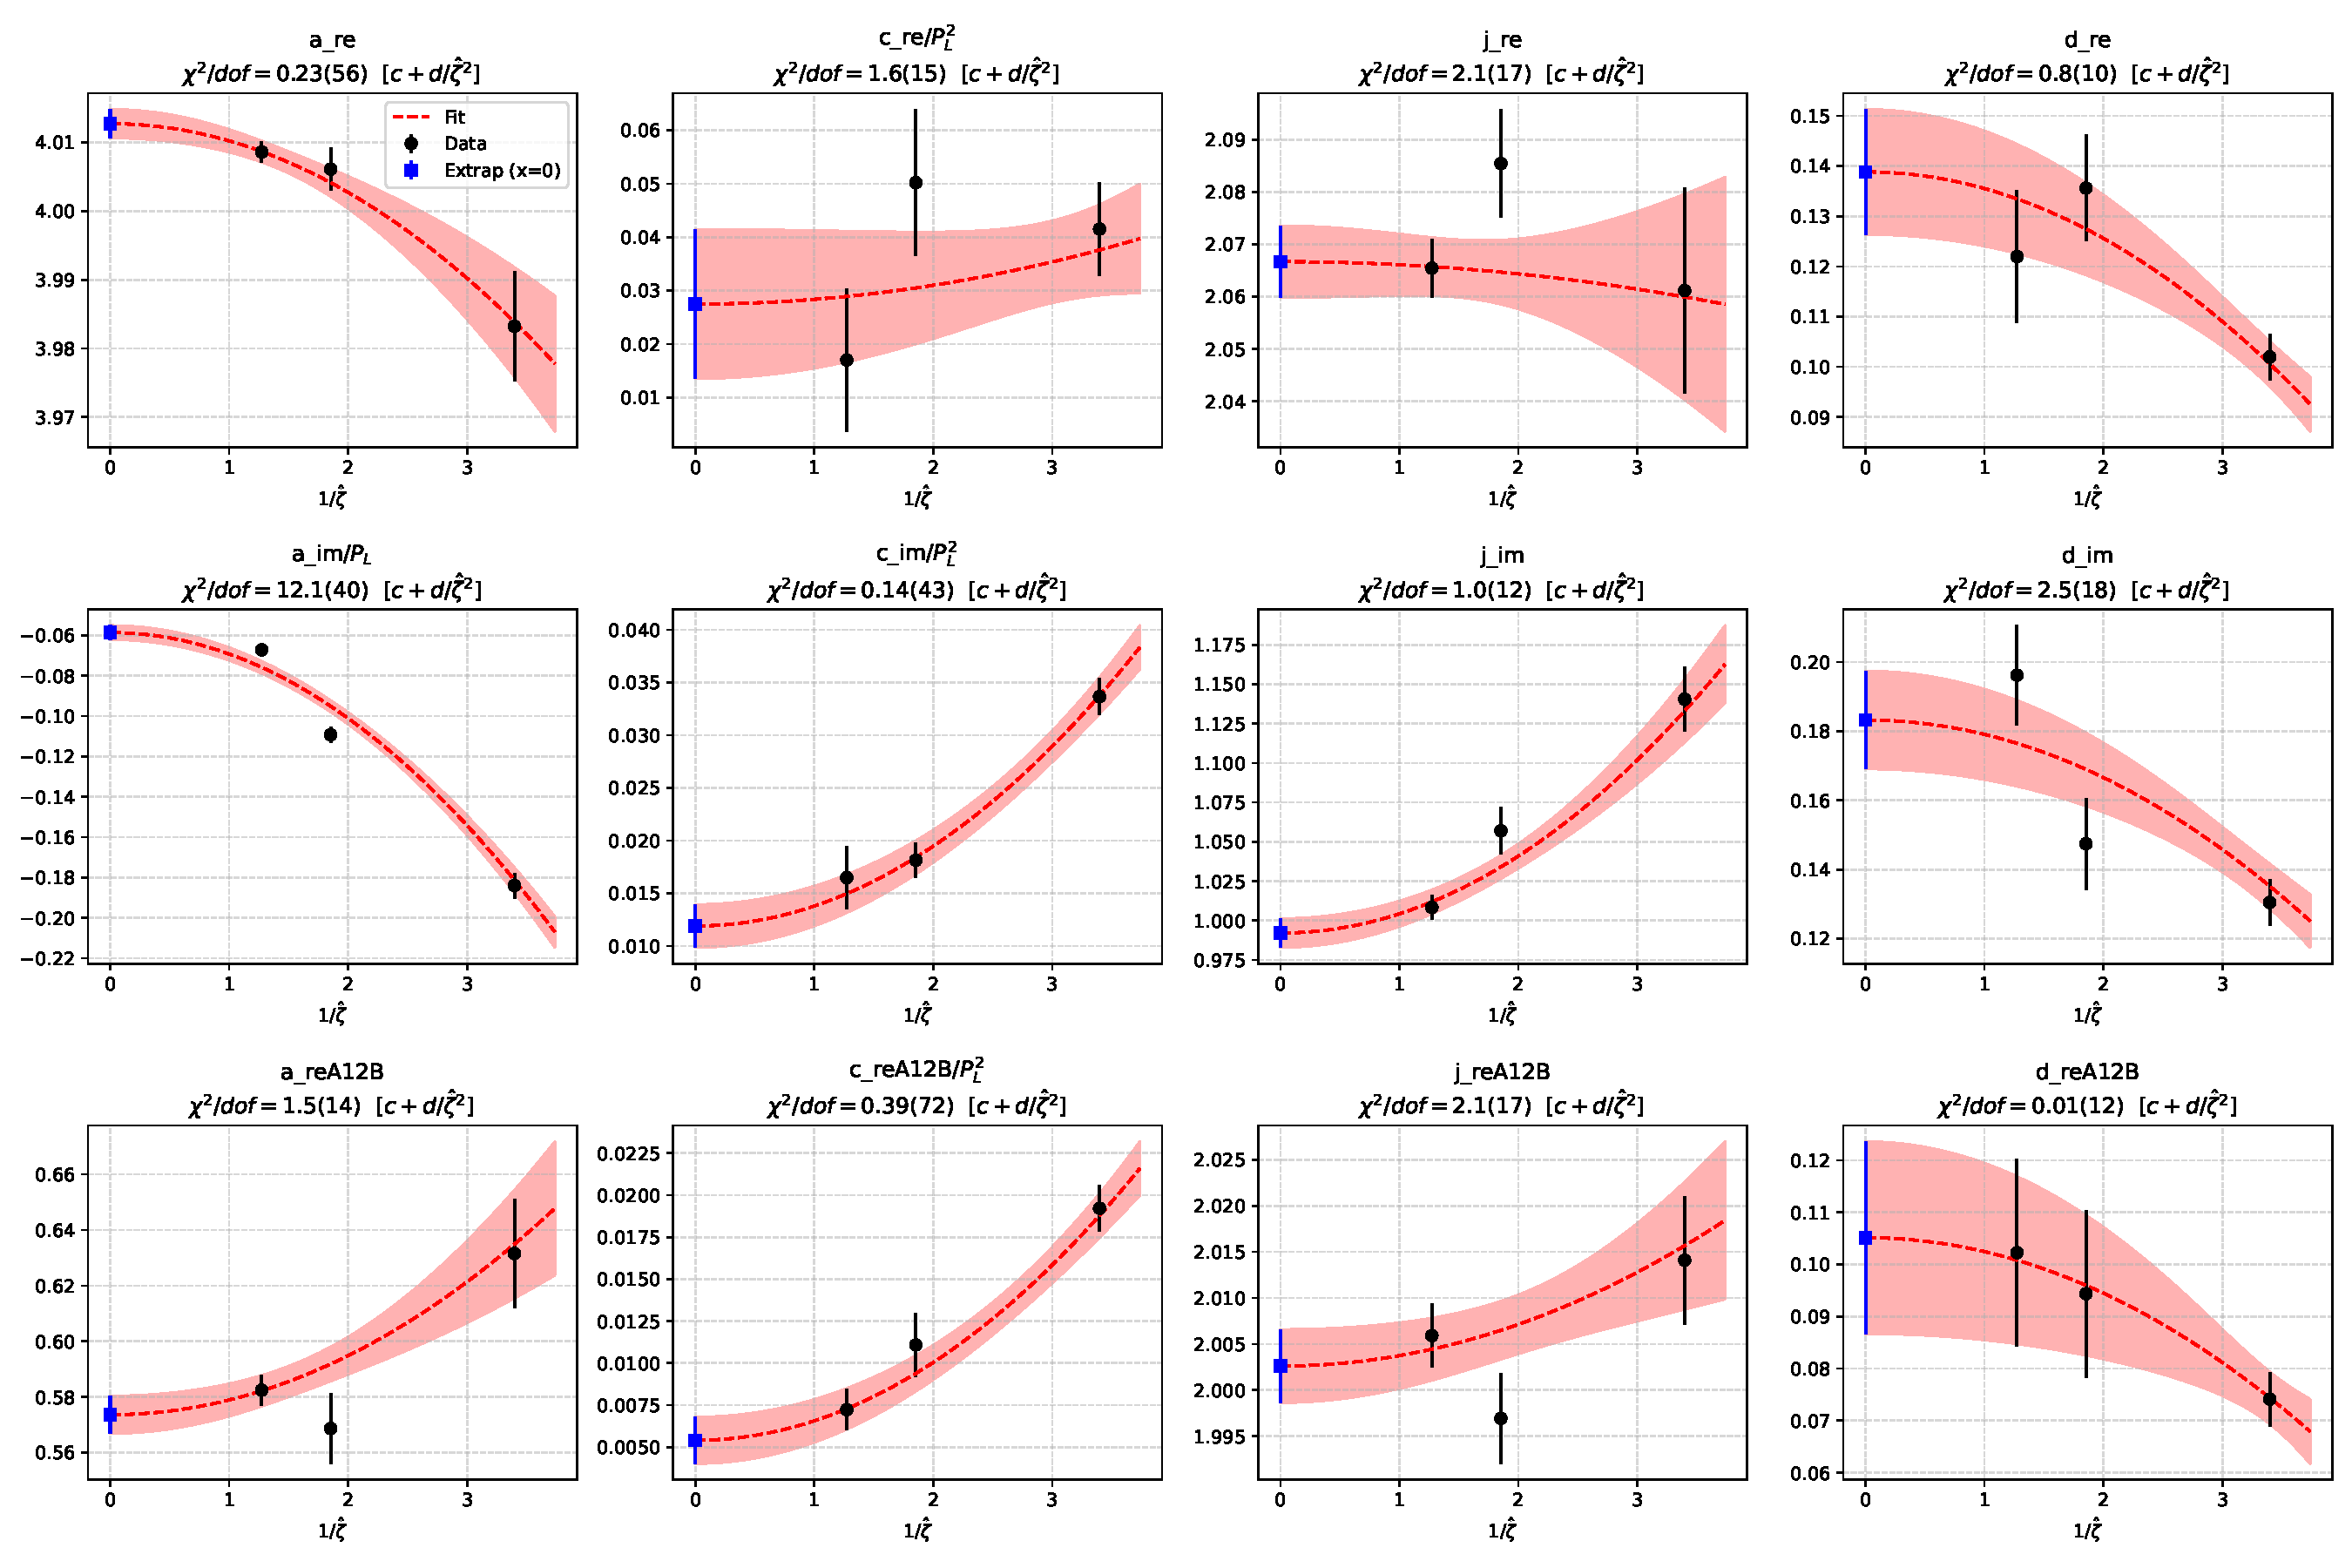
\includegraphics[height=0.68\textheight]{Param_Extrapolations_1byZetahat_sq_P234_bmin3_eta610_b29.0.pdf}\\
  {\scriptsize Twelve simultaneous-fit parameters vs $1/\hat\zeta$, using only $P_L=-2,-3,-4$ (black points). Dashed red curve and band: fitted ansatz $c+d/\hat\zeta^2$, with each panel's Jackknife $\chi^2/\mathrm{dof}$ in its title; blue square at $1/\hat\zeta=0$: extrapolated value. $c_{\rm re}$, $c_{\rm im}$ and $c_{\rm re}^{A_{12B}}$ are rescaled by $1/P_L^2$, $a_{\rm im}$ by $1/P_L$.}
\end{frame}

\begin{frame}{Amplitudes reconstructed at $\zetahat\to\infty$}
  \centering
  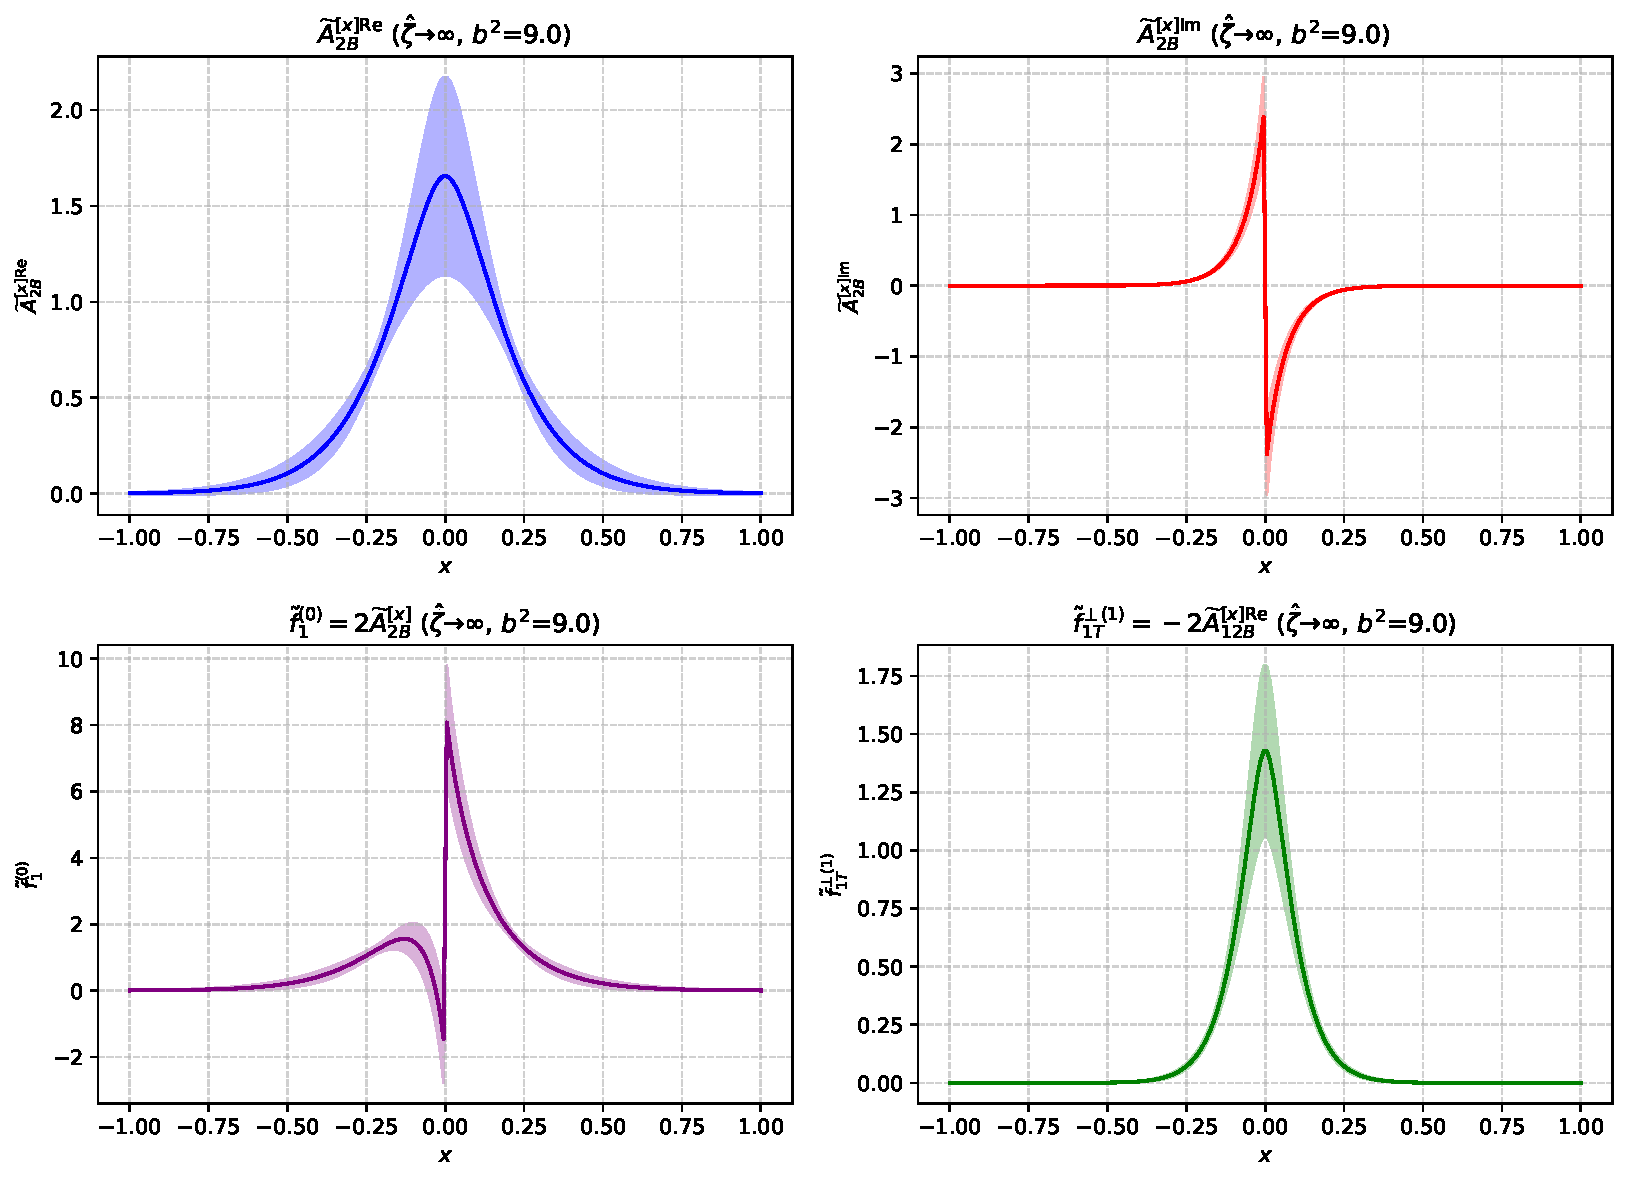
\includegraphics[height=0.68\textheight]{Extrapolated_AmpLevel_P234_Sivers_1_over_zetahat_sq_bmin3_eta610_b29.0_Amps.pdf}\\
  {\scriptsize $\tAmp^{[x]\text{Re}}_{2B}$, $\tAmp^{[x]\text{Im}}_{2B}$, $\tilde f_1^{(0)}=2\tAmp^{[x]}_{2B}$ and $\tilde f_{1T}^{\perp(1)}=-2\tAmp^{[x]\text{Re}}_{12B}$ from the extrapolated parameters, as continuous functions of $x$ at $|b_T|=3a\approx0.34$ fm. Bands: Jackknife uncertainty propagated from the twelve parameters.}
\end{frame}

\begin{frame}{Isovector ($u-d$) Sivers shift at $\zetahat\to\infty$}
  \centering
  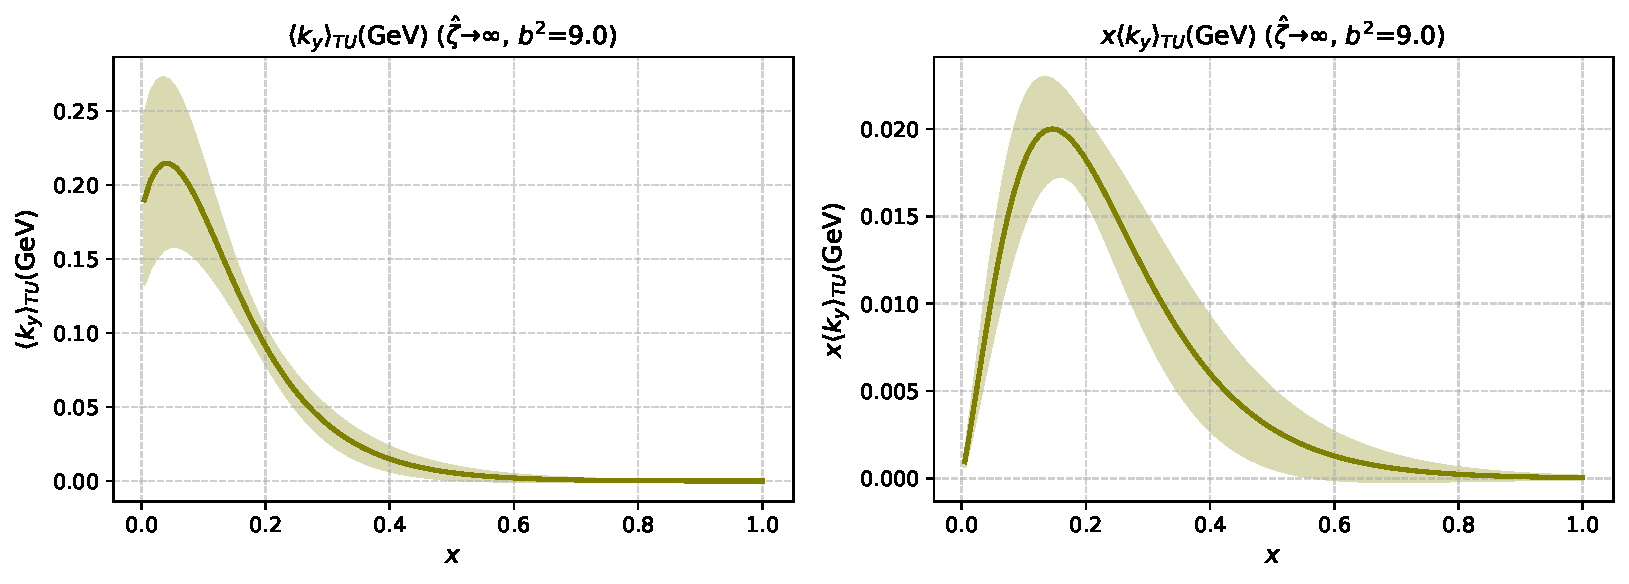
\includegraphics[width=\linewidth,height=0.6\textheight,keepaspectratio]{Extrapolated_AmpLevel_P234_Sivers_1_over_zetahat_sq_bmin3_eta610_b29.0_Sivers.pdf}\\
  {\scriptsize $\langle k_y\rangle_{TU}$ and $x\langle k_y\rangle_{TU}$ built from the extrapolated amplitudes of the previous slide, restricted to the quark region $x\ge0$. Bands: Jackknife uncertainty.}
\end{frame}

\begin{frame}{Numerical integration of the Fourier transforms at $\zetahat\to\infty$}
  \centering
  \renewcommand{\arraystretch}{1.8}
  \resizebox{\linewidth}{!}{\begin{tabular}{|l|c|c|c|c|}
  \hline
  Integral & $[-\infty, \infty]$ & $[-1, 1]$ & $[-1, 0]$ & $[0, 1]$ \\
  \hline
  $\int dx\, \tAmp^{[x]\text{Re}}_{2B}$ & $0.751(79)$ & $0.751(80)$ & $0.375(40)$ & $0.375(40)$ \\
  $\int dx\, (\tAmp^{[x]\text{Im}}_{2B})$ & $6(96)\times10^{-17}$ & $3(24)\times10^{-16}$ & $0.165(27)$ & $-0.169(29)$ \\
  $\int dx\, \tilde{f}_1^{(0)} = 2\int dx\, (\tAmp^{[x]\text{Re}}_{2B} - \tAmp^{[x]\text{Im}}_{2B})$ & $1.50(16)$ & $1.50(16)$ & $0.421(81)$ & $1.09(11)$ \\
  $\int dx\, \tilde{f}_{1T}^{\perp(1)} = -2\int dx\, \tAmp^{[x]\text{Re}}_{12B}$ & $0.302(53)$ & $0.302(53)$ & $0.151(27)$ & $0.151(27)$ \\
  $m_N \frac{\int dx\, \tilde{f}_{1T}^{\perp(1)}}{\int dx\, \tilde{f}_1^{(0)}}$ & $0.217(38)$ & $0.217(38)$ & $0.387(89)$ & $0.150(26)$ \\
  \hline
  \end{tabular}}\\[3mm]
  {\scriptsize At $|b_T|=3a\approx0.34$ fm, from the extrapolated ($\hat\zeta\to\infty$) amplitudes, over the full range and three restricted $x$-ranges isolating the quark, antiquark and combined contributions. The first four rows are unrenormalized; the multiplicative renormalization factor cancels only in the fifth row, where the ratio is formed.}
\end{frame}

\begin{frame}{Extrapolated amplitudes in $x=k^+/P^+$ and $|\vprp b|$}
  \centering
  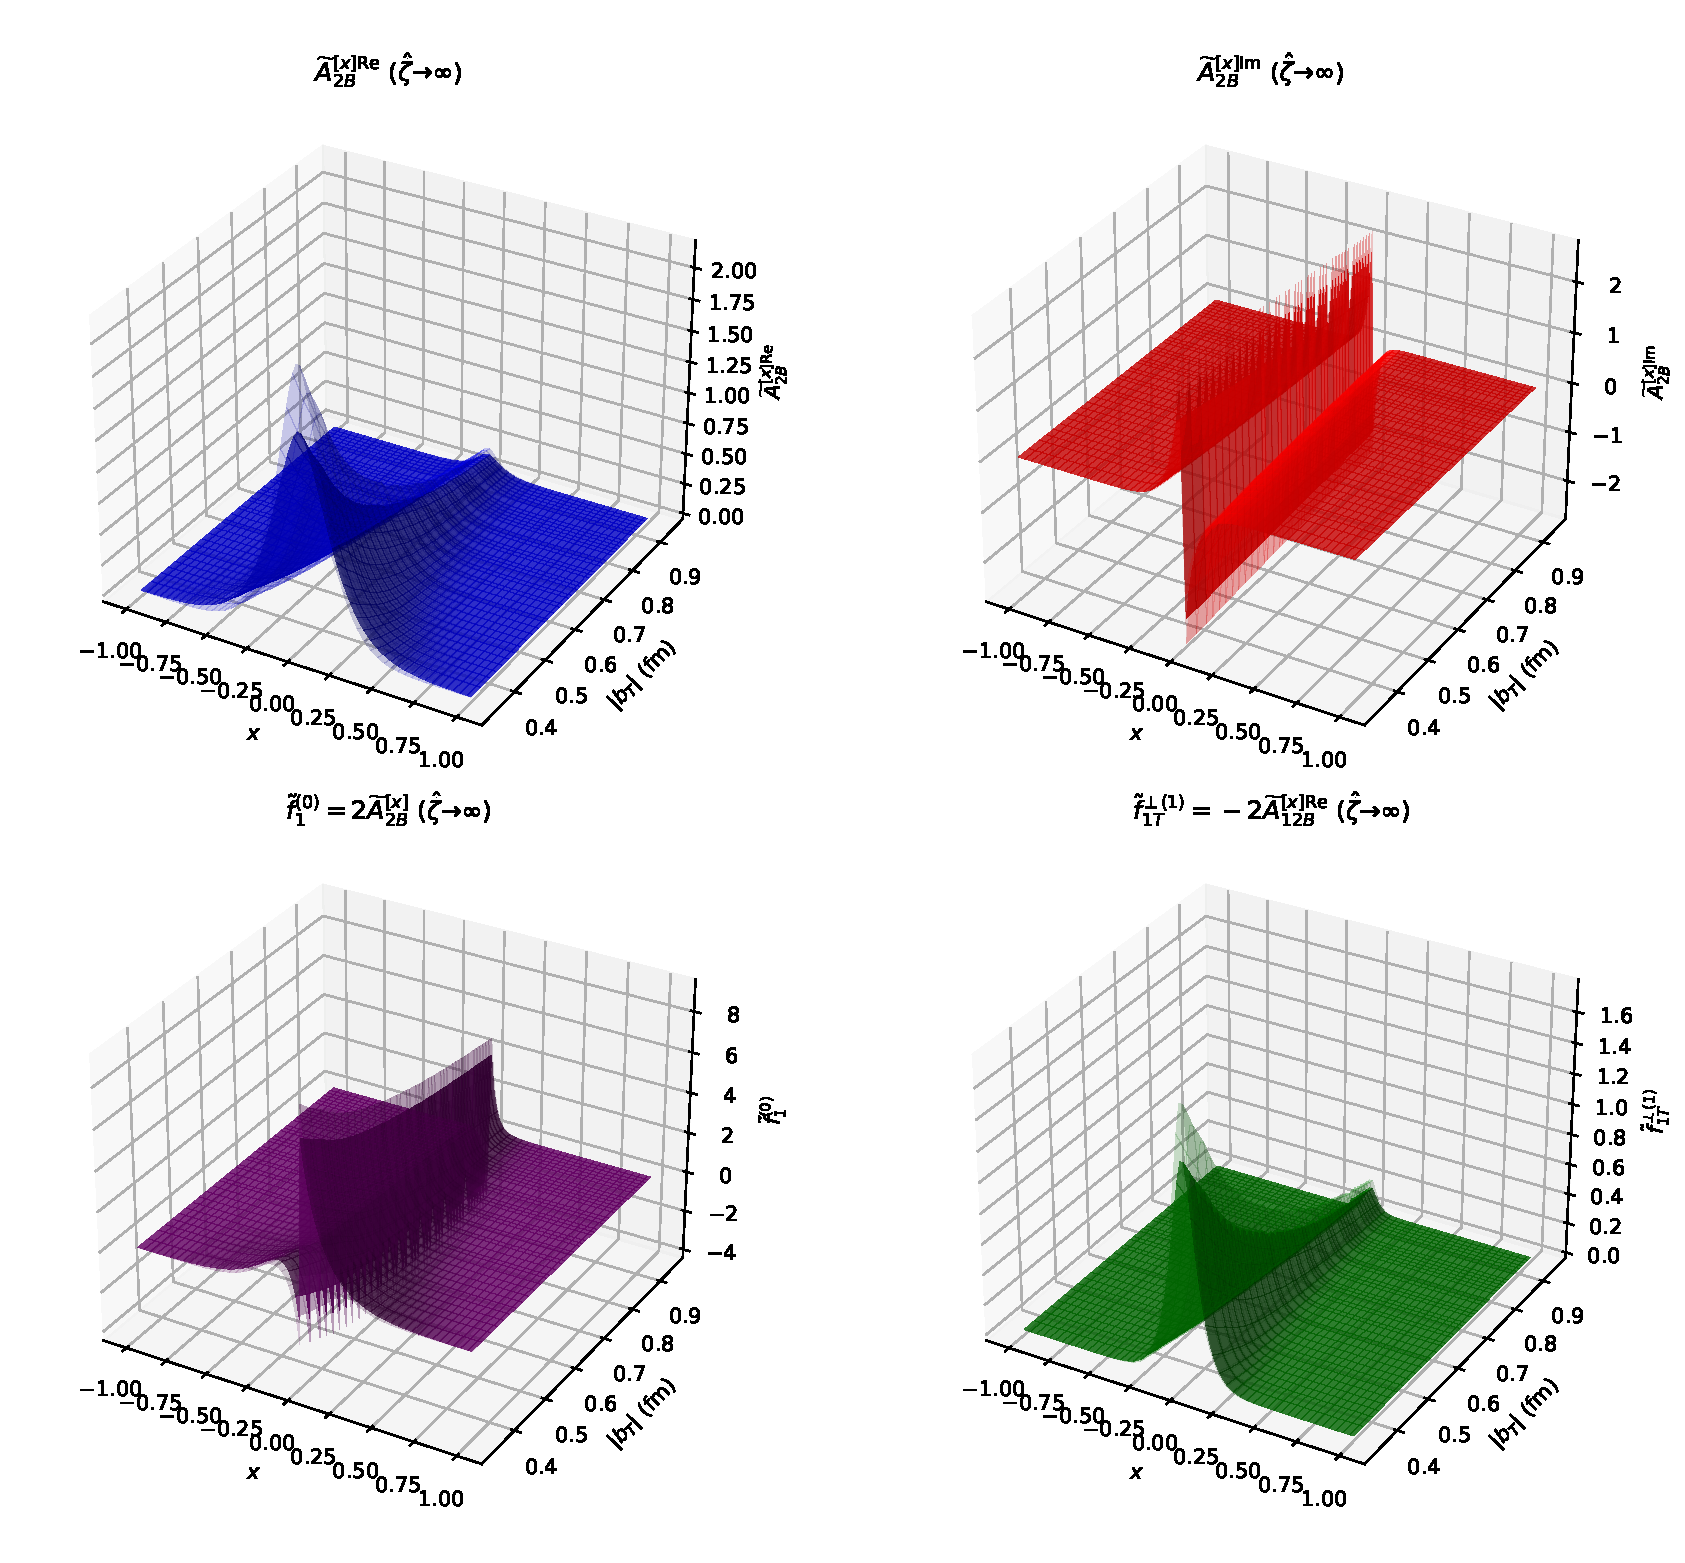
\includegraphics[height=0.68\textheight]{FT_xdep_3D_A2B_A12B_bmin3_eta610_PLInf_Amps.pdf}\\
  {\scriptsize The four extrapolated amplitude quantities as surfaces in $x$ and $|b_T|$ (from $3a\approx0.34$ fm to $\sqrt{68}\,a\approx0.94$ fm).}
\end{frame}

\begin{frame}{The isovector Sivers shift in $x=k^+/P^+$ and $|\vprp b|$}
  \centering
  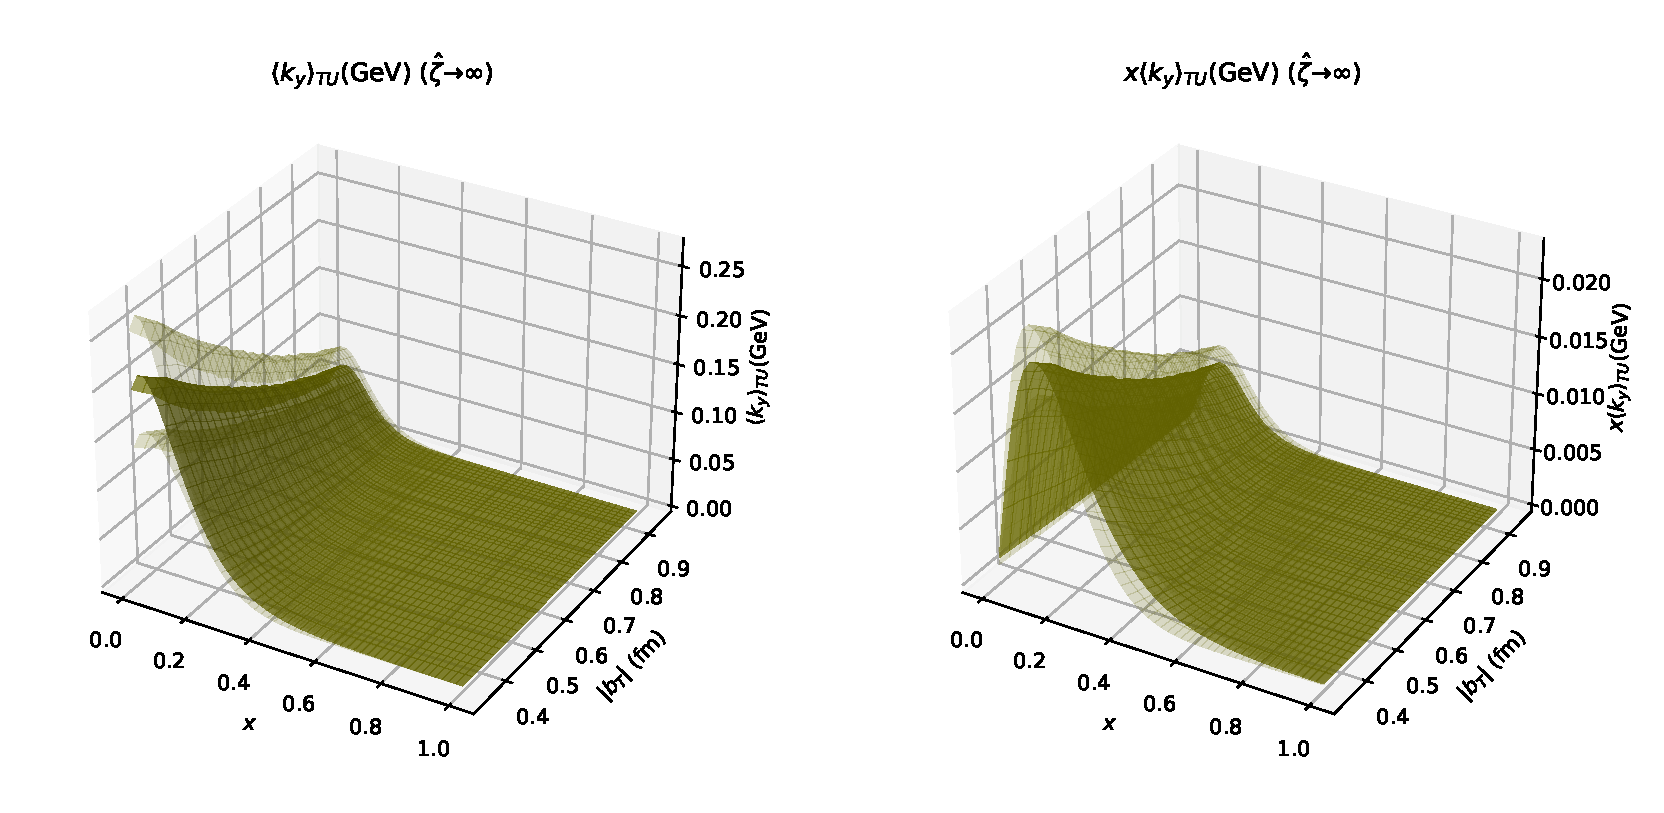
\includegraphics[width=0.95\linewidth,height=0.62\textheight,keepaspectratio]{FT_xdep_3D_A2B_A12B_bmin3_eta610_PLInf_Sivers.pdf}\\
  {\scriptsize The extrapolated isovector ($u-d$) Sivers shift $\langle k_y\rangle_{TU}$ and $x\langle k_y\rangle_{TU}$ as surfaces in $x\ge0$ and $|b_T|$, over the same range.}
\end{frame}

\begin{frame}{All four momenta against the extrapolated $\zetahat\to\infty$ result}
  \centering
  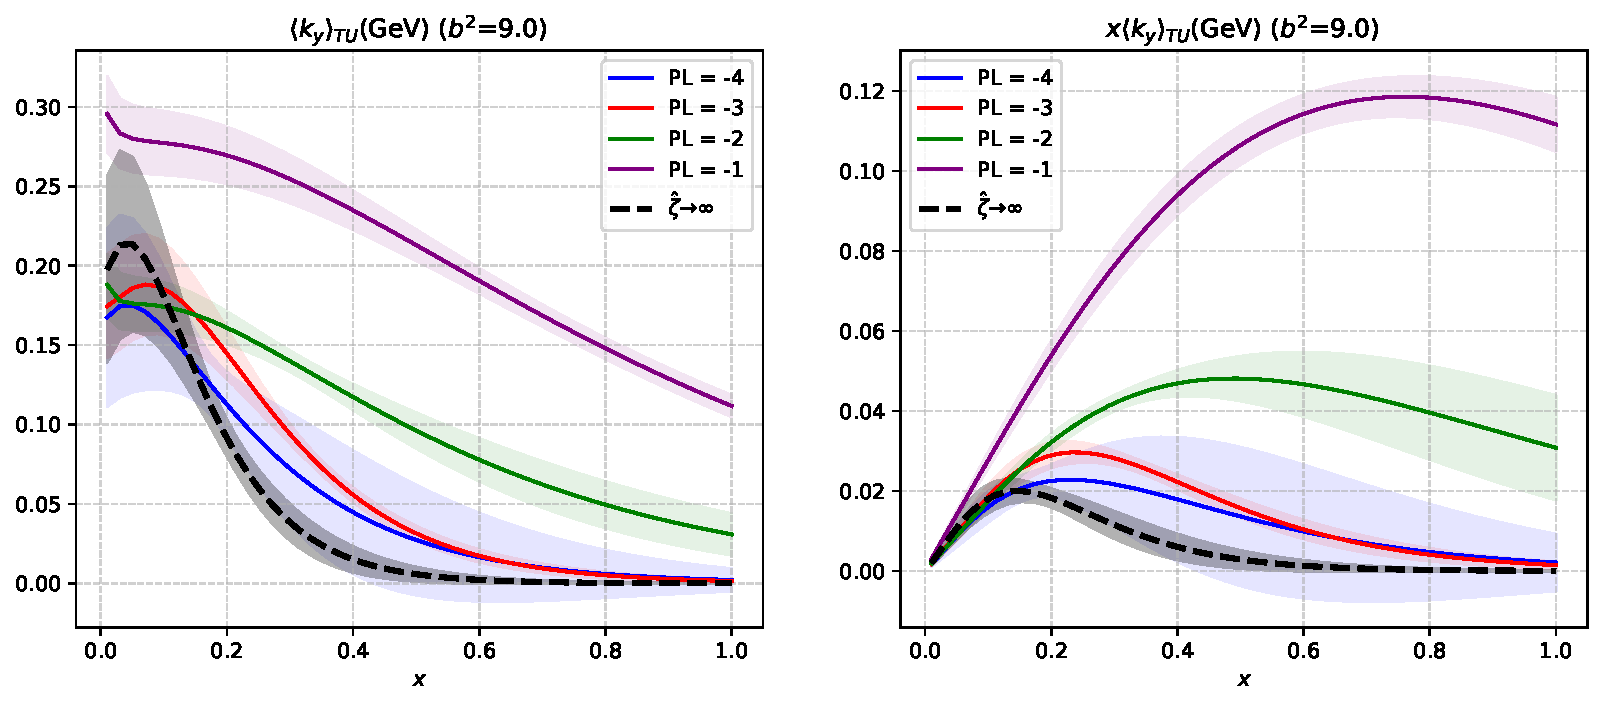
\includegraphics[width=0.9\linewidth]{All_Momenta_vs_Extrapolated_2D_P234_bmin3_eta610_b29.0_Sivers.pdf}
  \begin{itemize}
    \item $\langle k_y\rangle_{TU}$ and $x\langle k_y\rangle_{TU}$ at $|\vprp b|=3a\approx0.34$ fm change systematically from $P_L=-1$ to $-4$.
    \item The light-cone limit needs an extrapolation $\zetahat\to\infty$ (black dashed band).
  \end{itemize}
\end{frame}

% Slide 48
\begin{frame}{Ratio tests: is it factorized, $F(x)\,G(|\vprp b|)$?}
  \begin{columns}[c]
    \begin{column}{0.5\textwidth}
      \centering
      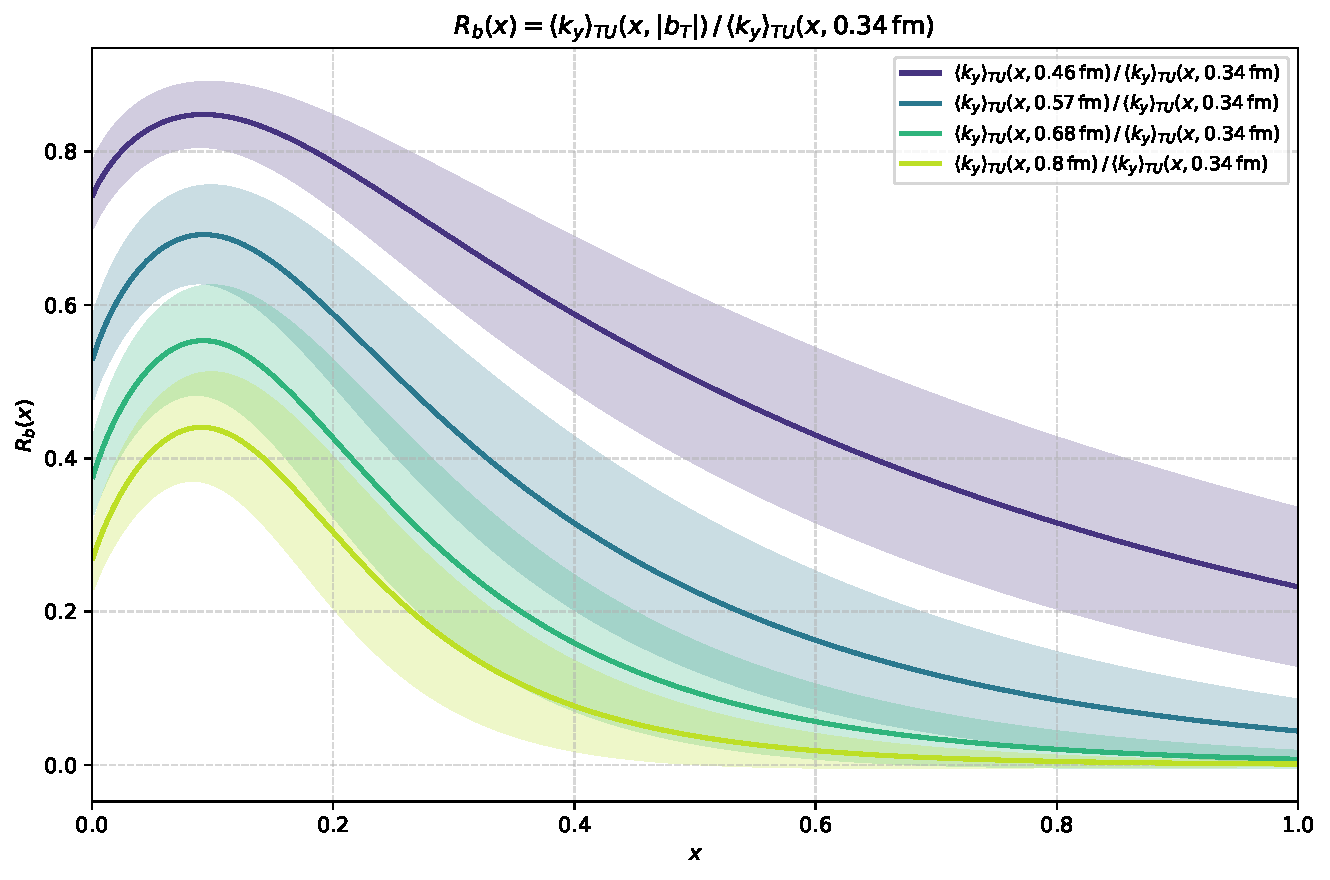
\includegraphics[width=\linewidth]{Factorization_Ratio_vs_x_4curves_P234_bmin3_eta610.pdf}\\
      {\scriptsize $R_b(x)=\langle k_y\rangle_{TU}(x,|\vprp b|)/\langle k_y\rangle_{TU}(x,0.34\,\text{fm})$: flat if factorized}
    \end{column}
    \begin{column}{0.48\textwidth}
      \centering
      relative distance $=\sqrt{J/N}$ of the best $F(x)G(|\vprp b|)$\\[1mm]
      {\small
      \begin{tabular}{cc}
        \toprule
        $x$-window & relative distance \\
        \midrule
        $[0.0,1.0]$ & $0.0568(78)$ \\
        $[0.1,0.9]$ & $0.0714(95)$ \\
        $[0.2,0.8]$ & $0.0758(75)$ \\
        $[0.3,0.8]$ & $0.0620(88)$ \\
        \bottomrule
      \end{tabular}}
      \begin{itemize}
        \item Isovector Sivers shift: $5.7$--$7.6\%$ from factorized; amplitudes: $8$--$19\%$ (for $x\in[0,1]$).
        \item The power $j$ is $\approx2$ for both real amplitudes but $\approx1$ for $\tAmp_{2B}^{\text{Im}}$.
      \end{itemize}
    \end{column}
  \end{columns}
  \keymsg{Close to factorized, but \textbf{not exactly}.}
\end{frame}
